\acao{Ação 3.2.2.6 – Esgotamento sanitário em propriedades de mananciais (área da SEAB)}

\pendencia{Ajuste do nome da ação (Orientações para elaboração dos cadernos, seção 6): “área do IDR-Paraná” passa a “área da SEAB”. A mesma alteração está registrada, em controle de alterações, no quadro de atividades e ações do Subcomponente 3.2. Informar à UGP.}

\phantomsection
\addcontentsline{toc}{subsection}{1. Contextualização}
\subsection*{1. Contextualização}

A ação implanta soluções individuais de esgotamento sanitário em 2.300 domicílios rurais situados em mananciais de abastecimento público da área prioritária do PSH-PR, em propriedades atendidas pela SEAB, entre 2029 e 2033. Além do atendimento a domicílios sem solução, a ação substitui sistemas inadequados de disposição do esgoto (IAT, 2026a).

O esgoto lançado sem tratamento no solo e nos cursos d'água de um manancial compromete a qualidade da água bruta destinada ao abastecimento público, com aporte de matéria orgânica, nutrientes e microrganismos patogênicos. Nos nove mananciais selecionados, 2.236 domicílios particulares permanentes ocupados apresentam destinação inadequada do esgoto, segundo os dados do Censo 2022 e do CNEFE (IAT, 2026a).

A ação reduz a carga poluidora nos mananciais e complementa a gestão de riscos nas bacias de abastecimento público, no próprio componente, e as práticas agropecuárias implantadas nas mesmas propriedades no Componente 2. Contribui também para o indicador de pessoas atendidas com, pelo menos, esgotamento sanitário, com cerca de 6,4 mil pessoas.

\textbf{Inclui:} a indicação dos domicílios pela SEAB; a contratação das soluções e das obras; o projeto sanitário de cada propriedade; a instalação conforme a ABNT NBR 17076:2024; a verificação técnica; a orientação do proprietário; e a medição, a comprovação e o pagamento, com validação técnica do IAT e da SEAB.

\textbf{Não inclui:} a elaboração dos Planos Integrados de Propriedade (PIP), realizada no Componente 2, nem redes coletoras ou intervenções no interior das moradias.

\textbf{Valor previsto:} R\$~18,40 milhões (empréstimo BIRD: R\$~18,40 milhões; contrapartida: R\$~0,00 milhões), conforme a planilha PSH\_CUSTO\_Consolidada.

\phantomsection
\addcontentsline{toc}{subsection}{2. Área de atuação}
\subsection*{2. Área de atuação}

A área de atuação resulta da aplicação sucessiva de critérios (Figura~\ref{selecao-mananciais}): microbacias prioritárias do PSH-PR; mananciais de abastecimento público selecionados por critérios de qualidade e de quantidade da água; domicílios rurais permanentes ocupados; ausência de destinação adequada do esgoto, segundo o Censo 2022; e existência de diagnóstico da microbacia e de adesão da propriedade ao PSH-PR e às ações da SEAB (IAT, 2026a).

\begin{figure}[H]
  \centering
  \caption{Critérios de seleção dos domicílios em mananciais}\label{selecao-mananciais}
  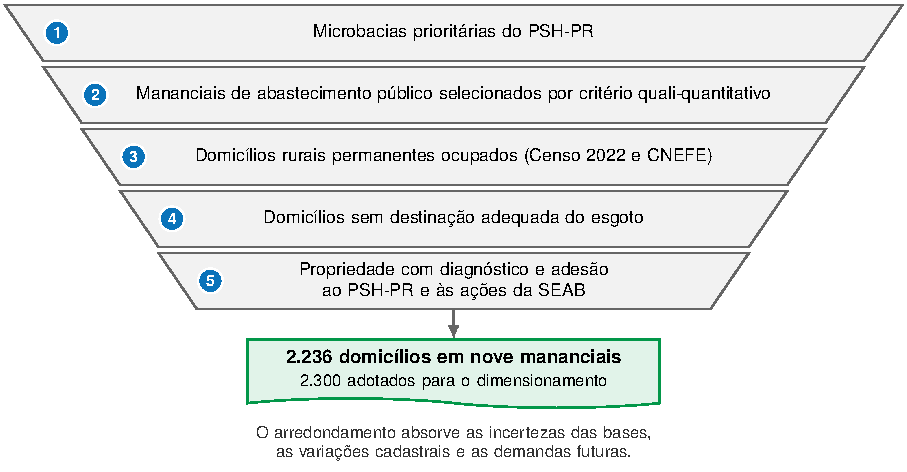
\includegraphics[width=15.37cm]{figuras/f-selecao-mananciais.pdf}
  \fonteMOP{Fonte: IAT (2026), com base em IAT (2026a).}
  % Texto alternativo: Funil com os cinco critérios de seleção dos domicílios em mananciais, que resulta em 2.236 domicílios e na meta de 2.300.
\end{figure}

A aplicação dos critérios resultou em 2.236 domicílios com esgotamento inadequado em nove mananciais, dos quais 1.925 no manancial do Rio Pirapó (Tabela~\ref{mananciais}). Para o dimensionamento da ação, o número foi arredondado para 2.300 domicílios, margem que absorve as incertezas das bases de dados, as variações cadastrais e as demandas futuras.

\begin{table}[H]
  \caption{Domicílios com esgotamento inadequado nos mananciais selecionados}\label{mananciais}
  \footnotesize\renewcommand{\arraystretch}{1.25}\setlength{\tabcolsep}{5pt}
  \begin{tabular}{>{\raggedright\arraybackslash}p{\dimexpr 0.3197\linewidth-2\tabcolsep\relax}>{\raggedright\arraybackslash}p{\dimexpr 0.2095\linewidth-2\tabcolsep\relax}>{\raggedleft\arraybackslash}p{\dimexpr 0.1874\linewidth-2\tabcolsep\relax}>{\raggedleft\arraybackslash}p{\dimexpr 0.1874\linewidth-2\tabcolsep\relax}>{\raggedleft\arraybackslash}p{\dimexpr 0.0960\linewidth-2\tabcolsep\relax}}
    \rowcolor{azulEscuro}\textcolor{white}{\textbf{Manancial}} & \textcolor{white}{\textbf{Critério}} & \centering\arraybackslash \textcolor{white}{\textbf{Domicílios permanentes}} & \centering\arraybackslash \textcolor{white}{\textbf{Esgotamento inadequado}} & \centering\arraybackslash \textcolor{white}{\textbf{\%}} \\
    Rio Marumbi & Qualitativo & 128 & 120 & 94 \\ \arrayrulecolor{cinza20}\hline
    \rowcolor{cinza5}Rio Pirapó & Qualitativo & 2.750 & 1.925 & 70 \\ \arrayrulecolor{cinza20}\hline
    Ribeirão Floresta & Qualitativo & 17 & 17 & 100 \\ \arrayrulecolor{cinza20}\hline
    \rowcolor{cinza5}Rio Palmital & Qualitativo & 20 & 16 & 80 \\ \arrayrulecolor{cinza20}\hline
    Ribeirão Paracatu & Qualitativo & 17 & 17 & 100 \\ \arrayrulecolor{cinza20}\hline
    \rowcolor{cinza5}Ribeirão Guarazinho & Qualitativo & 22 & 22 & 100 \\ \arrayrulecolor{cinza20}\hline
    Rio Água Grande & Qualitativo & 91 & 53 & 58 \\ \arrayrulecolor{cinza20}\hline
    \rowcolor{cinza5}Ribeirão Água na Campina & Qualitativo & 37 & 37 & 100 \\ \arrayrulecolor{cinza20}\hline
    Ribeirão do Noitimbo & Quali-quantitativo & 29 & 29 & 100 \\ \arrayrulecolor{cinza20}\hline
    \rowcolor{petroleo12}\textbf{Total} &  & \textbf{3.111} & \textbf{2.236} & \textbf{72} \\ \noalign{\global\arrayrulewidth=1pt}\arrayrulecolor{azulEscuro}\hline\noalign{\global\arrayrulewidth=0.4pt}
  \end{tabular}
  \fonteMOP{Fonte: Adaptado de IAT (2026a), com dados do Censo Demográfico 2022 agregados por setor censitário e do CNEFE (IBGE, 2024).}
  \notaMOP{Nota: domicílios particulares permanentes ocupados. Para o dimensionamento, adotaram-se 2.300 domicílios.}
\end{table}

\pendencia{Na tabela da nota técnica, o Rio Marumbi consta com 90\%, mas 120 de 128 domicílios correspondem a 94\%. Conferir.}

\pendencia{O Acordo de Empréstimo, item (j)(vii) das definições, exige a identificação das áreas rurais da Parte 3.2. Incluir o mapa dos nove mananciais, com as microbacias e os municípios.}

\phantomsection
\addcontentsline{toc}{subsection}{3. Arranjo institucional e partes interessadas}
\subsection*{3. Arranjo institucional e partes interessadas}

O IAT, por meio da DISAR, contrata a empresa, fiscaliza a instalação e efetua o pagamento, com apoio da supervisora das obras. A SEAB indica os domicílios a partir dos PIP, apoia a mobilização dos proprietários e participa da validação técnica dos resultados. A empresa contratada elabora o projeto de cada propriedade e executa a instalação, e o proprietário autoriza, acompanha e confirma a execução.

\begin{itemize}
  \item \textbf{Coexecutora:} SEAB, na indicação dos domicílios, na mobilização e na validação técnica;
  \item \textbf{Intervenientes:} empresa contratada; empresa supervisora das obras; UGP, que acompanha a execução;
  \item \textbf{Público envolvido:} proprietários e moradores das propriedades rurais dos mananciais.
\end{itemize}

Os beneficiários diretos são os moradores dos 2.300 domicílios, cerca de 6,4 mil pessoas. Os beneficiários indiretos são as populações abastecidas pelos mananciais, com a melhoria da qualidade da água bruta.

\phantomsection
\addcontentsline{toc}{subsection}{4. Processo de execução operacional}
\subsection*{4. Processo de execução operacional}

A ação adota o mesmo procedimento de instalação, verificação, medição e pagamento do esgotamento sanitário nas comunidades (Figura~\ref{instalacao} e Figura~\ref{medicao}), com as etapas por responsável apresentadas na Figura~\ref{raias-3226}. As diferenças referem-se à origem da demanda, ao território e à validação (Quadro~\ref{diferencas}): os domicílios são indicados pela SEAB a partir dos PIP, e não pelo trabalho técnico-social; o território corresponde aos mananciais de abastecimento público; e a validação técnica de cada lote conta com a participação da SEAB.

\begin{quadro}[H]
  \caption{Diferenças entre as ações de esgotamento sanitário}\label{diferencas}
  \footnotesize\renewcommand{\arraystretch}{1.25}\setlength{\tabcolsep}{5pt}
  \begin{tabular}{>{\raggedright\arraybackslash}p{\dimexpr 0.2425\linewidth-2\tabcolsep\relax}>{\raggedright\arraybackslash}p{\dimexpr 0.3787\linewidth-2\tabcolsep\relax}>{\raggedright\arraybackslash}p{\dimexpr 0.3788\linewidth-2\tabcolsep\relax}}
    \rowcolor{azulEscuro}\textcolor{white}{\textbf{Aspecto}} & \textcolor{white}{\textbf{Esgotamento sanitário nas comunidades}} & \textcolor{white}{\textbf{Esgotamento sanitário em mananciais}} \\
    Origem da demanda & Diagnóstico do trabalho técnico-social & PIP, com indicação dos domicílios pela SEAB \\ \arrayrulecolor{cinza20}\hline
    \rowcolor{cinza5}Território & Comunidades atendidas pelos sistemas de abastecimento de água & Nove mananciais da área prioritária do PSH-PR \\ \arrayrulecolor{cinza20}\hline
    Base do levantamento & Censo 2022 e CNEFE: 70\% dos 5.810 domicílios sem esgotamento adequado & Censo 2022 e CNEFE: 2.236 domicílios, arredondados para 2.300 \\ \arrayrulecolor{cinza20}\hline
    \rowcolor{cinza5}Meta & 4.067 domicílios & 2.300 domicílios \\ \arrayrulecolor{cinza20}\hline
    Prazo & 2028 a 2033 & 2029 a 2033 \\ \arrayrulecolor{cinza20}\hline
    \rowcolor{cinza5}Validação & IAT & IAT, com a SEAB \\ \noalign{\global\arrayrulewidth=1pt}\arrayrulecolor{azulEscuro}\hline\noalign{\global\arrayrulewidth=0.4pt}
  \end{tabular}
  \fonteMOP{Fonte: IAT (2026), com base em IAT (2026a) e PARANÁ (2026).}
\end{quadro}

\begin{figure}[H]
  \centering
  \caption{Fluxograma do esgotamento sanitário em mananciais: entradas, etapas por responsável e saídas}\label{raias-3226}
  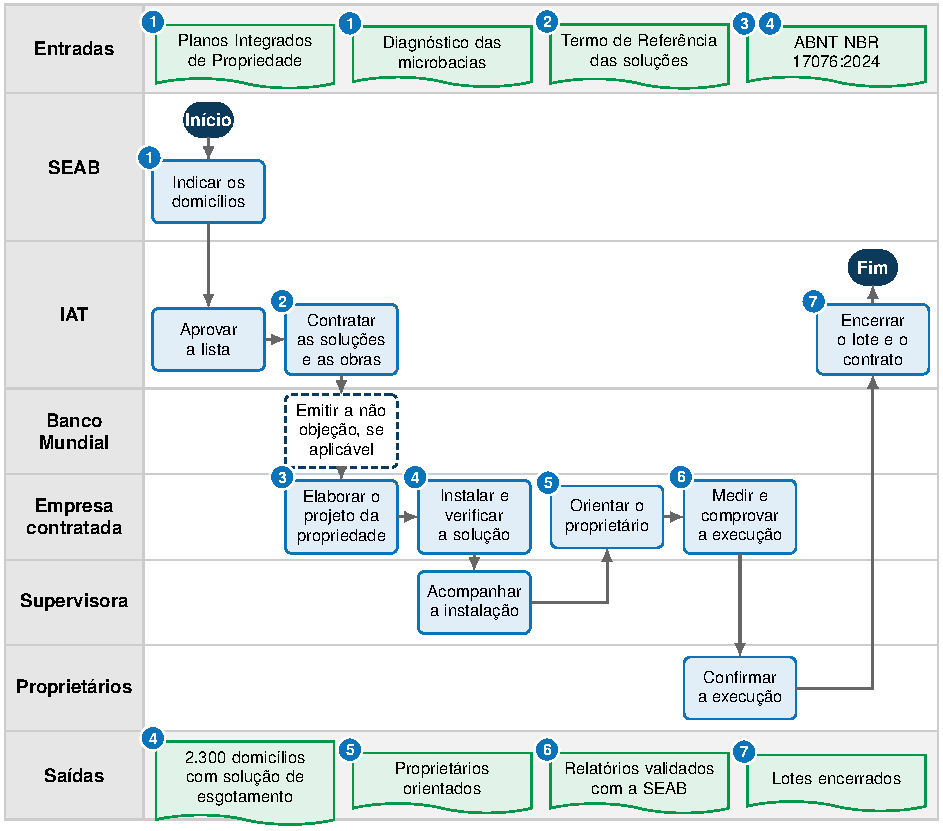
\includegraphics[width=15.96cm]{figuras/g-raias-3226.pdf}
  \fonteMOP{Fonte: IAT (2026).}
  % Texto alternativo: Fluxograma em raias do esgotamento sanitário em mananciais, com uma raia por instituição, as etapas numeradas na raia do executor, as entradas no topo e as saídas na base.
\end{figure}

\phantomsection
\subsubsection*{4.1 Etapa 1: Indicação dos domicílios pela SEAB}

\textbf{Atividades:} indicação pela SEAB, a partir dos PIP e do diagnóstico das microbacias, dos domicílios sem destinação adequada do esgoto; confirmação da adesão e autorização da intervenção pelo proprietário.

\textbf{Entradas:} PIP; diagnóstico das microbacias; critérios do item 2.

\textbf{Responsáveis:} SEAB (executa); IAT (aprova a lista); proprietários (consultados).

\textbf{Produto:} lista de domicílios por manancial.

\pendencia{Confirmar o cronograma dos PIP no Componente 2, que condiciona o início das instalações em 2029.}

\phantomsection
\subsubsection*{4.2 Etapa 2: Contratação das soluções e das obras}

\textbf{Atividades:} elaboração do Termo de Referência das soluções descentralizadas e das obras civis; publicação do edital; licitação; contratação. A contratação pode integrar o processo do esgotamento sanitário nas comunidades, em lotes próprios.

\textbf{Entradas:} lista de domicílios; especificações conforme a ABNT NBR 17076:2024.

\textbf{Responsáveis:} IAT (executa e aprova); SEAB (consultada); UGP e Banco Mundial (consultados, quando houver revisão prévia).

\textbf{Produto:} contrato assinado.

\phantomsection
\subsubsection*{4.3 Etapa 3: Projeto sanitário da propriedade}

\textbf{Atividades:} elaboração, pela empresa contratada, do projeto de cada propriedade, considerada a topografia do terreno, o número de moradores, a capacidade de infiltração do solo e a solução de tratamento adequada, inclusive o manejo do lodo.

\textbf{Entradas:} contrato; dados do PIP.

\textbf{Responsáveis:} empresa contratada (executa); IAT (aprova); SEAB e proprietário (consultados).

\textbf{Produto:} projeto aprovado.

\phantomsection
\subsubsection*{4.4 Etapa 4: Instalação e verificação técnica}

\textbf{Atividades:} execução das obras civis e instalação dos dispositivos; verificação do funcionamento, da estanqueidade e da garantia; correções, quando necessárias, conforme a Figura~\ref{instalacao}.

\textbf{Entradas:} projeto aprovado; autorização do proprietário.

\textbf{Responsáveis:} empresa contratada (executa); supervisora (acompanha); IAT (aprova).

\textbf{Produto:} sistema verificado e validado.

\phantomsection
\subsubsection*{4.5 Etapa 5: Orientação do proprietário}

\textbf{Atividades:} orientação quanto ao funcionamento, ao uso adequado, à manutenção preventiva e à limpeza periódica, durante a instalação, com apoio da equipe técnica da SEAB que atende a propriedade.

\textbf{Entradas:} sistema em instalação; material de orientação.

\textbf{Responsáveis:} empresa contratada (executa); SEAB (consultada); IAT (aprova o material).

\textbf{Produto:} proprietário orientado.

\phantomsection
\subsubsection*{4.6 Etapa 6: Medição, comprovação e pagamento}

\textbf{Atividades:} relatórios de medição e evidências; assinatura do proprietário; auditoria documental e verificação \textit{in loco}; relatório de medição final; amostragem \textit{in loco}; ordenação da despesa e pagamento, conforme a Figura~\ref{medicao}. O IAT aprova cada lote após a validação técnica realizada com a SEAB.

\textbf{Entradas:} sistemas validados; assinaturas dos proprietários.

\textbf{Responsáveis:} empresa contratada (executa); SEAB (consultada na validação); IAT (aprova e efetua o pagamento).

\textbf{Produto:} relatório técnico aprovado pelo IAT, com a validação da SEAB, e comprovante de pagamento, por lote.

\pendencia{A nota técnica prevê validação conjunta. Na matriz, a SEAB figura como C (consultada antes da aprovação), porque o Guia de Identidade Visual admite um único A por etapa. Confirmar o papel com a SEAB e registrá-lo no protocolo de validação.}

\phantomsection
\subsubsection*{4.7 Etapa 7: Encerramento}

\textbf{Atividades:} encerramento de cada lote e do contrato; registro das propriedades atendidas, para a assistência técnica prestada pela SEAB.

\textbf{Entradas:} relatórios aprovados e pagamentos realizados.

\textbf{Responsáveis:} IAT (executa); UGP (valida).

\textbf{Produto:} lote encerrado.

\phantomsection
\subsubsection*{4.8 Modalidade de execução}

O item de custo é o sistema individual de tratamento de efluentes: 2.300 domicílios a R\$~8.000,00, no total de R\$~18,40 milhões, com recursos do empréstimo do BIRD. A execução ocorre mediante licitação de obras, com o projeto e a instalação no mesmo contrato, conforme o Caderno AQ. O eventual agrupamento com o esgotamento sanitário nas comunidades em um mesmo processo, em lotes distintos, é definido no Plano de Aquisições.

\phantomsection
\addcontentsline{toc}{subsection}{5. Matriz de responsabilidades}
\subsection*{5. Matriz de responsabilidades}

O Quadro~\ref{raci-3226} apresenta o papel de cada parte em cada etapa.

\begin{quadro}[H]
  \caption{Matriz de responsabilidades do esgotamento sanitário em mananciais}\label{raci-3226}
  \footnotesize\renewcommand{\arraystretch}{1.25}\setlength{\tabcolsep}{3pt}
  \begin{tabular}{>{\raggedright\arraybackslash}p{\dimexpr 0.2536\linewidth-2\tabcolsep\relax}>{\centering\arraybackslash}p{\dimexpr 0.0882\linewidth-2\tabcolsep\relax}>{\centering\arraybackslash}p{\dimexpr 0.0882\linewidth-2\tabcolsep\relax}>{\centering\arraybackslash}p{\dimexpr 0.0882\linewidth-2\tabcolsep\relax}>{\centering\arraybackslash}p{\dimexpr 0.0882\linewidth-2\tabcolsep\relax}>{\centering\arraybackslash}p{\dimexpr 0.0882\linewidth-2\tabcolsep\relax}>{\centering\arraybackslash}p{\dimexpr 0.0882\linewidth-2\tabcolsep\relax}>{\centering\arraybackslash}p{\dimexpr 0.0882\linewidth-2\tabcolsep\relax}>{\centering\arraybackslash}p{\dimexpr 0.1291\linewidth-2\tabcolsep\relax}}
    \rowcolor{azulEscuro}\textcolor{white}{\textbf{Parte}} & \textcolor{white}{\textbf{E1}} & \textcolor{white}{\textbf{E2}} & \textcolor{white}{\textbf{E3}} & \textcolor{white}{\textbf{E4}} & \textcolor{white}{\textbf{E5}} & \textcolor{white}{\textbf{E6}} & \textcolor{white}{\textbf{E7}} & \textcolor{white}{\textbf{Produto final}} \\
    IAT & \raci{A} & \raci{R} \raci{A} & \raci{A} & \raci{A} & \raci{A} & \raci{A} & \raci{R} & \raci{A} \\ \arrayrulecolor{cinza20}\hline
    \rowcolor{cinza5}SEAB & \raci{R} & \raci{C} & \raci{C} & \raci{I} & \raci{C} & \raci{C} & \raci{I} & \raci{C} \\ \arrayrulecolor{cinza20}\hline
    Empresa contratada & – & – & \raci{R} & \raci{R} & \raci{R} & \raci{R} & \raci{I} & \raci{R} \\ \arrayrulecolor{cinza20}\hline
    \rowcolor{cinza5}Supervisora & – & – & – & \raci{R} & – & \raci{C} & – & – \\ \arrayrulecolor{cinza20}\hline
    Proprietários & \raci{C} & – & \raci{C} & \raci{I} & \raci{R} & \raci{R} & \raci{I} & \raci{I} \\ \arrayrulecolor{cinza20}\hline
    \rowcolor{cinza5}UGP & \raci{I} & \raci{C} & \raci{I} & \raci{I} & \raci{I} & \raci{I} & \raci{A} & \raci{I} \\ \arrayrulecolor{cinza20}\hline
    Banco Mundial & – & \raci{C} & – & – & – & – & – & – \\ \noalign{\global\arrayrulewidth=1pt}\arrayrulecolor{azulEscuro}\hline\noalign{\global\arrayrulewidth=0.4pt}
  \end{tabular}
  \fonteMOP{Fonte: IAT (2026).}
  \notaMOP{Nota: E1 a E7 correspondem às Etapas 1 a 7 do item 4. \raci{R} executa (pode haver mais de um); \raci{A} aprova ou valida o produto (um por etapa); \raci{C} é consultado previamente; \raci{I} é informado posteriormente. Produto final: domicílios dos mananciais com solução individual instalada e aprovada.}
\end{quadro}

\phantomsection
\addcontentsline{toc}{subsection}{6. Metas, indicadores e comprovação}
\subsection*{6. Metas, indicadores e comprovação}

A meta é de 460 domicílios por ano, de 2029 a 2033 (Quadro~\ref{metas-3226}).

\begin{quadro}[H]
  \caption{Metas anuais do esgotamento sanitário em mananciais}\label{metas-3226}
  \footnotesize\renewcommand{\arraystretch}{1.25}\setlength{\tabcolsep}{3pt}
  \begin{tabular}{>{\raggedright\arraybackslash}p{\dimexpr 0.2095\linewidth-2\tabcolsep\relax}>{\raggedright\arraybackslash}p{\dimexpr 0.1268\linewidth-2\tabcolsep\relax}>{\raggedleft\arraybackslash}p{\dimexpr 0.0794\linewidth-2\tabcolsep\relax}>{\raggedleft\arraybackslash}p{\dimexpr 0.0794\linewidth-2\tabcolsep\relax}>{\raggedleft\arraybackslash}p{\dimexpr 0.0794\linewidth-2\tabcolsep\relax}>{\raggedleft\arraybackslash}p{\dimexpr 0.0794\linewidth-2\tabcolsep\relax}>{\raggedleft\arraybackslash}p{\dimexpr 0.0794\linewidth-2\tabcolsep\relax}>{\raggedleft\arraybackslash}p{\dimexpr 0.0794\linewidth-2\tabcolsep\relax}>{\raggedleft\arraybackslash}p{\dimexpr 0.0794\linewidth-2\tabcolsep\relax}>{\raggedleft\arraybackslash}p{\dimexpr 0.1081\linewidth-2\tabcolsep\relax}}
    \rowcolor{azulEscuro}\textcolor{white}{\textbf{Produto}} & \textcolor{white}{\textbf{Unidade}} & \centering\arraybackslash \textcolor{white}{\textbf{Ano 1}} & \centering\arraybackslash \textcolor{white}{\textbf{Ano 2}} & \centering\arraybackslash \textcolor{white}{\textbf{Ano 3}} & \centering\arraybackslash \textcolor{white}{\textbf{Ano 4}} & \centering\arraybackslash \textcolor{white}{\textbf{Ano 5}} & \centering\arraybackslash \textcolor{white}{\textbf{Ano 6}} & \centering\arraybackslash \textcolor{white}{\textbf{Ano 7}} & \centering\arraybackslash \textcolor{white}{\textbf{Total}} \\
    Sistema individual de tratamento de efluentes & domicílios & – & – & 460 & 460 & 460 & 460 & 460 & 2.300 \\ \noalign{\global\arrayrulewidth=1pt}\arrayrulecolor{azulEscuro}\hline\noalign{\global\arrayrulewidth=0.4pt}
  \end{tabular}
  \fonteMOP{Fonte: Planilha PSH\_CUSTO\_Consolidada, versão v2408 (PARANÁ, 2026).}
  \notaMOP{Nota: Ano 1 = 2027 e Ano 7 = 2033.}
\end{quadro}

Os indicadores constam do Quadro~\ref{ind-3226}; o de pessoas atendidas é calculado da mesma forma que no esgotamento sanitário nas comunidades.

\begin{quadro}[H]
  \caption{Indicadores do esgotamento sanitário em mananciais}\label{ind-3226}
  \footnotesize\renewcommand{\arraystretch}{1.25}\setlength{\tabcolsep}{3pt}
  \begin{tabular}{>{\raggedright\arraybackslash}p{\dimexpr 0.3165\linewidth-2\tabcolsep\relax}>{\raggedright\arraybackslash}p{\dimexpr 0.1378\linewidth-2\tabcolsep\relax}>{\raggedleft\arraybackslash}p{\dimexpr 0.1102\linewidth-2\tabcolsep\relax}>{\raggedleft\arraybackslash}p{\dimexpr 0.1599\linewidth-2\tabcolsep\relax}>{\raggedright\arraybackslash}p{\dimexpr 0.2756\linewidth-2\tabcolsep\relax}}
    \rowcolor{azulEscuro}\textcolor{white}{\textbf{Indicador}} & \textcolor{white}{\textbf{Unidade}} & \centering\arraybackslash \textcolor{white}{\textbf{Linha de base (2025)}} & \centering\arraybackslash \textcolor{white}{\textbf{Meta}} & \textcolor{white}{\textbf{Frequência e fonte dos dados}} \\
    Domicílios de mananciais com solução individual instalada e aprovada & domicílios & 0 & 2.300 & Por lote; IAT e SEAB \\ \arrayrulecolor{cinza20}\hline
    \rowcolor{cinza5}Pessoas atendidas com, pelo menos, esgotamento sanitário (parcela do indicador do componente) & pessoas & 0 & 6.440 & Anual; IAT, com desagregação por sexo e jovens \\ \arrayrulecolor{cinza20}\hline
    Mananciais com instalações concluídas & mananciais & 0 & 9 & Anual; IAT \\ \noalign{\global\arrayrulewidth=1pt}\arrayrulecolor{azulEscuro}\hline\noalign{\global\arrayrulewidth=0.4pt}
  \end{tabular}
  \fonteMOP{Fonte: IAT (2026).}
\end{quadro}

Os critérios de aceite são os mesmos do esgotamento sanitário nas comunidades, com validação técnica realizada com a SEAB (Quadro~\ref{aceite-3226}).

\begin{quadro}[H]
  \caption{Critérios de aceite e evidências do esgotamento sanitário em mananciais}\label{aceite-3226}
  \footnotesize\renewcommand{\arraystretch}{1.25}\setlength{\tabcolsep}{5pt}
  \begin{tabular}{>{\raggedright\arraybackslash}p{\dimexpr 0.2150\linewidth-2\tabcolsep\relax}>{\raggedright\arraybackslash}p{\dimexpr 0.3386\linewidth-2\tabcolsep\relax}>{\raggedright\arraybackslash}p{\dimexpr 0.2921\linewidth-2\tabcolsep\relax}>{\raggedright\arraybackslash}p{\dimexpr 0.1543\linewidth-2\tabcolsep\relax}}
    \rowcolor{azulEscuro}\textcolor{white}{\textbf{Produto}} & \textcolor{white}{\textbf{Critério de aceite}} & \textcolor{white}{\textbf{Evidência de comprovação}} & \textcolor{white}{\textbf{Responsável pela validação}} \\
    Lista de domicílios & Domicílios dos mananciais sem destinação adequada, com adesão do proprietário & Lista da SEAB, com os PIP de origem & IAT \\ \arrayrulecolor{cinza20}\hline
    \rowcolor{cinza5}Projeto sanitário & Solução adequada à propriedade, conforme a ABNT NBR 17076:2024 & Projeto aprovado & IAT \\ \arrayrulecolor{cinza20}\hline
    Sistema instalado & Execução conforme o projeto; teste de estanqueidade aprovado & Relatório de medição; laudo de verificação; registro fotográfico & IAT, com a SEAB \\ \arrayrulecolor{cinza20}\hline
    \rowcolor{cinza5}Execução confirmada & Execução confirmada pelo proprietário & Assinatura do proprietário & IAT \\ \arrayrulecolor{cinza20}\hline
    Lote aprovado & Auditoria documental, verificação \textit{in loco} e amostragem aprovadas & Relatório técnico aprovado; comprovante de pagamento & IAT, com a SEAB \\ \noalign{\global\arrayrulewidth=1pt}\arrayrulecolor{azulEscuro}\hline\noalign{\global\arrayrulewidth=0.4pt}
  \end{tabular}
  \fonteMOP{Fonte: IAT (2026).}
\end{quadro}

\phantomsection
\addcontentsline{toc}{subsection}{7. Gestão de riscos e impactos ambientais e sociais}
\subsection*{7. Gestão de riscos e impactos ambientais e sociais}

Os riscos são os mesmos do esgotamento sanitário nas comunidades, com atenção adicional à proteção dos recursos hídricos, por se tratar de instalações em mananciais de abastecimento público (Quadro~\ref{nas-3226}).

\begin{quadro}[H]
  \caption{Aplicação das Normas Ambientais e Sociais ao esgotamento sanitário em mananciais}\label{nas-3226}
  \footnotesize\renewcommand{\arraystretch}{1.25}\setlength{\tabcolsep}{5pt}
  \begin{tabular}{>{\raggedright\arraybackslash}p{\dimexpr 0.1874\linewidth-2\tabcolsep\relax}>{\raggedright\arraybackslash}p{\dimexpr 0.3716\linewidth-2\tabcolsep\relax}>{\raggedright\arraybackslash}p{\dimexpr 0.4410\linewidth-2\tabcolsep\relax}}
    \rowcolor{azulEscuro}\textcolor{white}{\textbf{NAS}} & \textcolor{white}{\textbf{Aplicação à ação}} & \textcolor{white}{\textbf{Medidas e instrumentos}} \\
    NAS 1 – Avaliação e gestão de riscos & Instalação em propriedades de mananciais & Dimensionamento conforme a ABNT NBR 17076:2024; distâncias mínimas de nascentes e cursos d'água; verificação técnica (MGAS) \\ \arrayrulecolor{cinza20}\hline
    \rowcolor{cinza5}NAS 2 – Condições de trabalho & Trabalhadores das empresas contratadas & Uso de EPI; treinamento de segurança; Procedimentos de Gestão de Mão de Obra \\ \arrayrulecolor{cinza20}\hline
    NAS 3 – Eficiência de recursos e prevenção da poluição & Contaminação do solo e da água do manancial; lodo & Testes de estanqueidade; orientação sobre o manejo do lodo; Plano de Gerenciamento de Resíduos Sólidos \\ \arrayrulecolor{cinza20}\hline
    \rowcolor{cinza5}NAS 4 – Saúde e segurança da comunidade & Valas abertas nas propriedades & Sinalização, isolamento e proteção das valas \\ \arrayrulecolor{cinza20}\hline
    NAS 10 – Engajamento das partes interessadas & Proprietários rurais & Autorização prévia; apoio da equipe técnica da SEAB; Mecanismo de Queixas e Reclamações (PEPI e MQR) \\ \noalign{\global\arrayrulewidth=1pt}\arrayrulecolor{azulEscuro}\hline\noalign{\global\arrayrulewidth=0.4pt}
  \end{tabular}
  \fonteMOP{Fonte: IAT (2026), com base nos instrumentos do Caderno AS.}
  \notaMOP{Nota: a NAS 5 não se aplica, por não haver aquisição de terras; a NAS 6 é verificada na triagem das propriedades situadas em áreas de preservação.}
\end{quadro}

\phantomsection
\addcontentsline{toc}{subsection}{8. Cronograma}
\subsection*{8. Cronograma}

A SEAB indica os domicílios a partir de 2028, a contratação ocorre em 2029 e as instalações estendem-se de 2029 a 2033, com 460 domicílios por ano (Figura~\ref{crono-3226}).

\begin{figure}[H]
  \centering
  \caption{Cronograma das etapas e das entregas do esgotamento sanitário em mananciais}\label{crono-3226}
  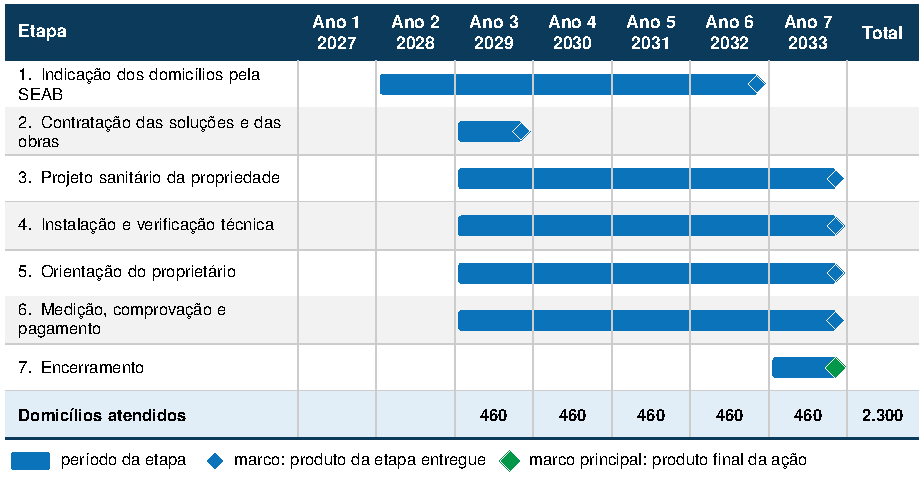
\includegraphics[width=15.64cm]{figuras/g-crono-3226.pdf}
  \fonteMOP{Fonte: IAT (2026), com quantidades da planilha PSH\_CUSTO\_Consolidada (PARANÁ, 2026).}
  % Texto alternativo: Cronograma anual de 2027 a 2033 com as etapas e as quantidades a entregar do esgotamento sanitário em mananciais.
\end{figure}

\phantomsection
\addcontentsline{toc}{subsection}{9. Interfaces e dependências}
\subsection*{9. Interfaces e dependências}

A ação depende dos PIP e do diagnóstico das microbacias, elaborados no Componente 2, e da supervisão das instalações. Fornece à gestão de riscos nas bacias de abastecimento a redução da carga de esgoto nos mananciais, à UGP o número de pessoas atendidas para o indicador do componente e à SEAB o registro das propriedades atendidas (Figura~\ref{interf-3226}).

\begin{figure}[H]
  \centering
  \caption{Interfaces e dependências do esgotamento sanitário em mananciais}\label{interf-3226}
  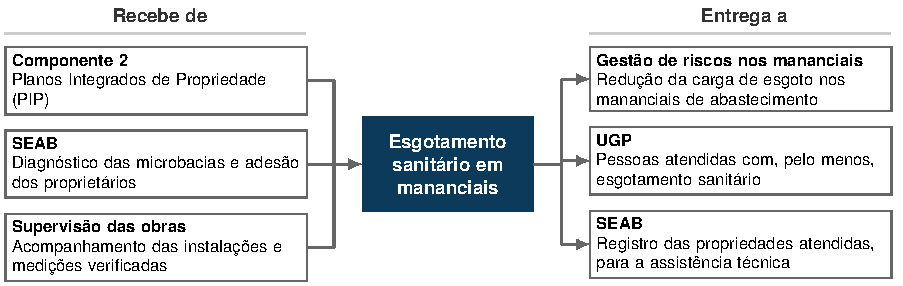
\includegraphics[width=15.30cm]{figuras/g-interf-3226.pdf}
  \fonteMOP{Fonte: IAT (2026).}
  % Texto alternativo: Diagrama das interfaces do esgotamento sanitário em mananciais: insumos recebidos de outras partes do Programa e produtos entregues a elas.
\end{figure}

\phantomsection
\addcontentsline{toc}{subsection}{10. Documentos complementares}
\subsection*{10. Documentos complementares}

\begin{itemize}
  \item ABNT NBR 17076:2024 (ABNT, 2024);
  \item Planos Integrados de Propriedade (Componente 2);
  \item Protocolo de validação técnica IAT–SEAB (a elaborar);
  \item Termo de Referência e edital das soluções e das obras (a elaborar);
  \item Caderno AQ e Caderno AS.
\end{itemize}
